\documentclass[pdflatex,compress,mathserif]{beamer}

%\usetheme[dark,framenumber,totalframenumber]{ElektroITK}
\usetheme[darktitle,framenumber,totalframenumber]{ElektroITK}

\usepackage[utf8]{inputenc}
\usepackage[T1]{fontenc}
\usepackage{lmodern}
\usepackage[english]{babel}
\usepackage{amsmath}
\usepackage{amsfonts}
\usepackage{amssymb}
\usepackage{graphicx}
\usepackage{multicol}
\usepackage{lipsum}
\usepackage{framed}
\usefonttheme[onlymath]{serif}

\newcommand*{\Scale}[2][4]{\scalebox{#1}{$#2$}}%

\setbeamertemplate{caption}[numbered]

\title{Digital Signal Processing}

\subtitle{Sampling}

\date{August, $7^{th}$ 2023}

\author{Mifta Nur Farid}

\begin{document}

\maketitle

\section{Sampling of continuos signal}

\begin{frame}{A digital signal processing scheme}
    \begin{figure}
        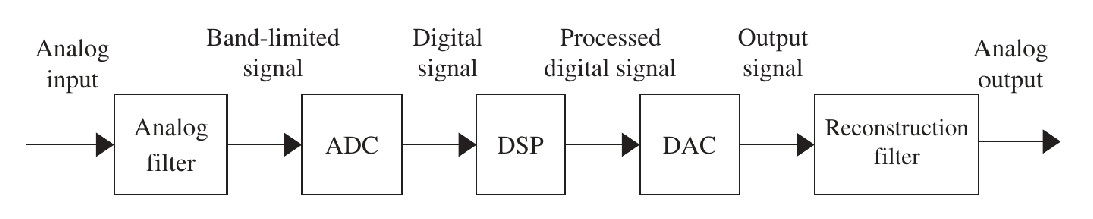
\includegraphics[width=\linewidth]{./img/img01.png}
    \end{figure}
\end{frame}

\begin{frame}{Sampling of continuos signal}
    \begin{itemize}
        \item The analog signal contains an infinite number of points
        \item The infinite points are not appropriate to be processed by a digital signal processor or a computer
    \end{itemize}
\end{frame}

\begin{frame}{Sampling of continuos signal}
    \begin{itemize}
        \item Sampling can solve such a problem by taking samples at the fixed time interval, where the time $T$ represents the sampling interval or sampling period in seconds.
        \begin{figure}
            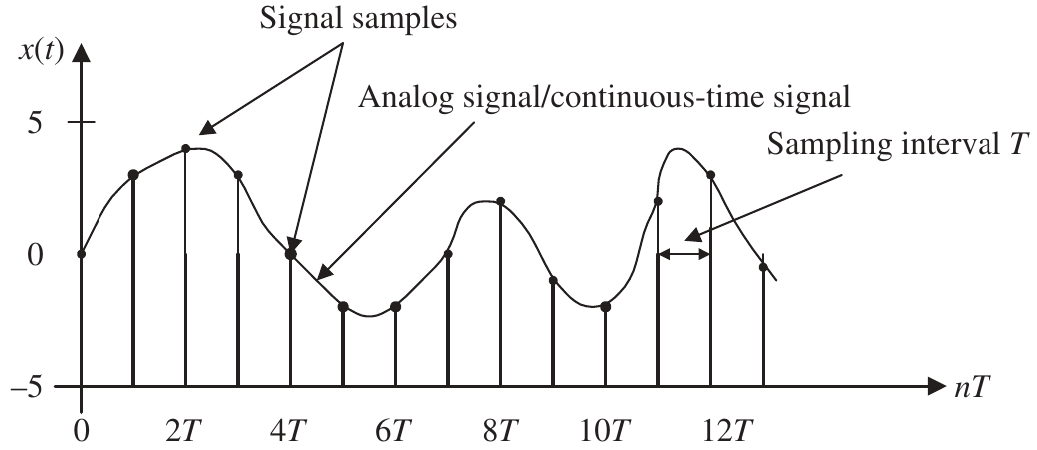
\includegraphics[width=0.8\linewidth]{./img/img02.png}
        \end{figure}
    \end{itemize}
\end{frame}

\begin{frame}{Sample-and-hold analog\\voltage for ADC}
    \begin{itemize}
        \item Each sample maintains its voltage level during the sampling interval T to give
        the ADC enough time to convert it.
        \item This process is called \textbf{sample and hold}
        \begin{figure}
            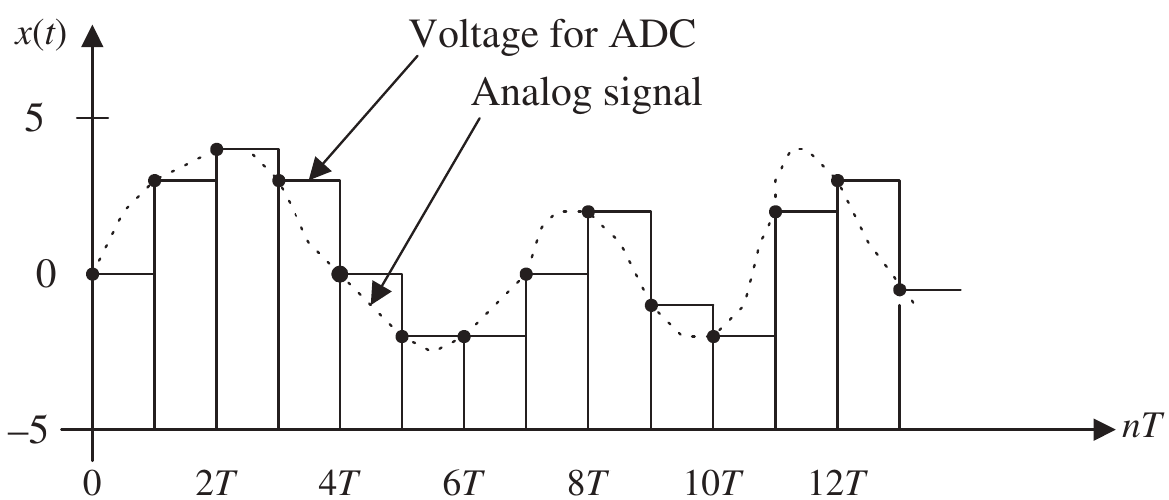
\includegraphics[width=0.9\linewidth]{./img/img03.png}
        \end{figure}
    \end{itemize}
\end{frame}

\begin{frame}{Sampling rate}
    \begin{itemize}
        \item For a given sampling interval $T$, which is defined as the time span between two neighboring sample points, the sampling rate is therefore given by
        \begin{equation*}
            f_s = \frac{1}{T} \text{ samples per second (Hz)}
        \end{equation*}
        \item For example, if a sampling period is $T = 125 \mu s$, the sampling rate is determined as $$f_s = 1/125 \mu s = 8000 \text{ samples per second (Hz) }$$ .
    \end{itemize}
\end{frame}

\begin{frame}{Sampling rate}
    \begin{itemize}
        \item After the analog signal is sampled, we obtain the sampled signal whose amplitude values are taken at the sampling instants, thus the processor is able to handle the sample points.
        \item  Next, we have to ensure that samples are collected at a rate high enough that the original analog signal can be reconstructed or recovered later.
    \end{itemize}    
\end{frame}

\begin{frame}{Sampling rate}
    \begin{itemize}
        \item In other words, we are looking for a minimum sampling rate to acquire a complete reconstruction of the analog signal from its sampled version
        \item If an analog signal is not appropriately sampled, \textbf{aliasing} will occur, which causes unwanted signals in the desired frequency band
    \end{itemize}    
\end{frame}

\begin{frame}{Sampling rate}
    \begin{itemize}
        \item The sampling theorem guarantees that an analog signal can be in theory perfectly recovered as long as the \textbf{sampling rate is at least twice} of the highest-frequency component of the analog signal to be sampled.
        $$f_s \geq 2 f_\text{max}$$ 
    \end{itemize}    
\end{frame}

\begin{frame}{Sampling rate}
    \begin{itemize}
        \item A sine wave with a frequency of 40 Hz and its sampled amplitudes
        \item The sampling interval between sample points is $T = 0.01 \text{ s}$, thus the sampling rate is $f_s = \frac{1}{T} = \frac{1}{0.01} = 100 \text{ Hz}$
        \item The sampling theorem condition is satisfied since $2f_\text{max} =  80 < f_s$
        \begin{figure}
            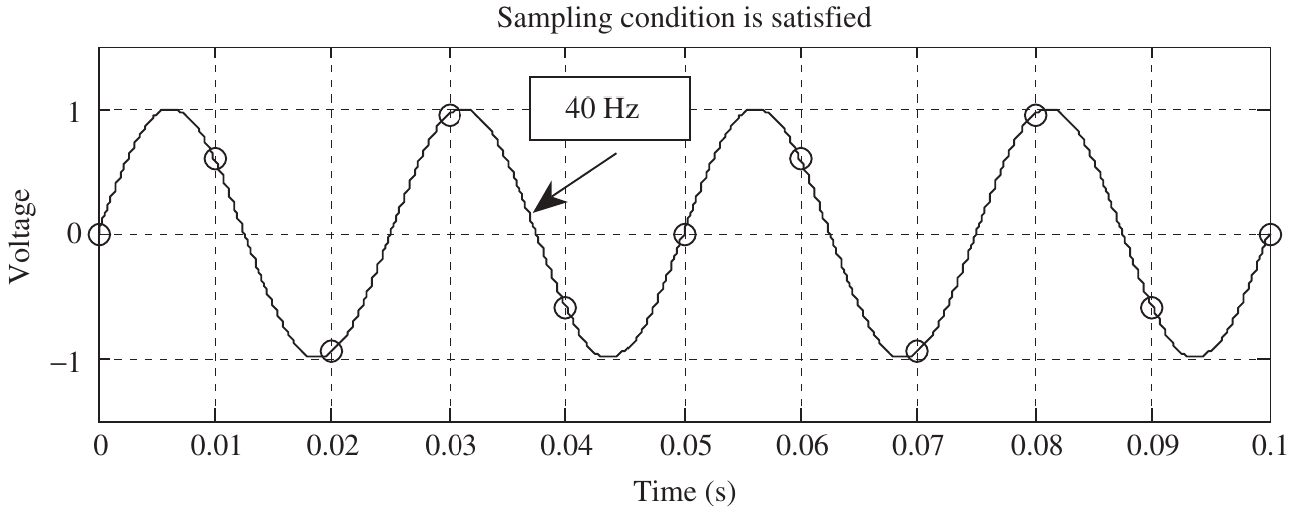
\includegraphics[width=0.9\linewidth]{./img/img04.png}
        \end{figure}
    \end{itemize}
\end{frame}

\begin{frame}{Sampling rate}
    \begin{itemize}
        \item The sine wave with a frequency of 90 Hz is sampled at 100 Hz
        \item The signal is undersampled due to $2f_\text{max} = 180 > f_s$
        \item We cannot tell whether the sampled signal comes from sampling a 90-Hz sine wave or from sampling a 10-Hz sine wave
        \item  They are not distinguishable. Thus they are \textbf{aliases} of each other. The 10-Hz sine wave is the aliasing noise.
        \begin{figure}
            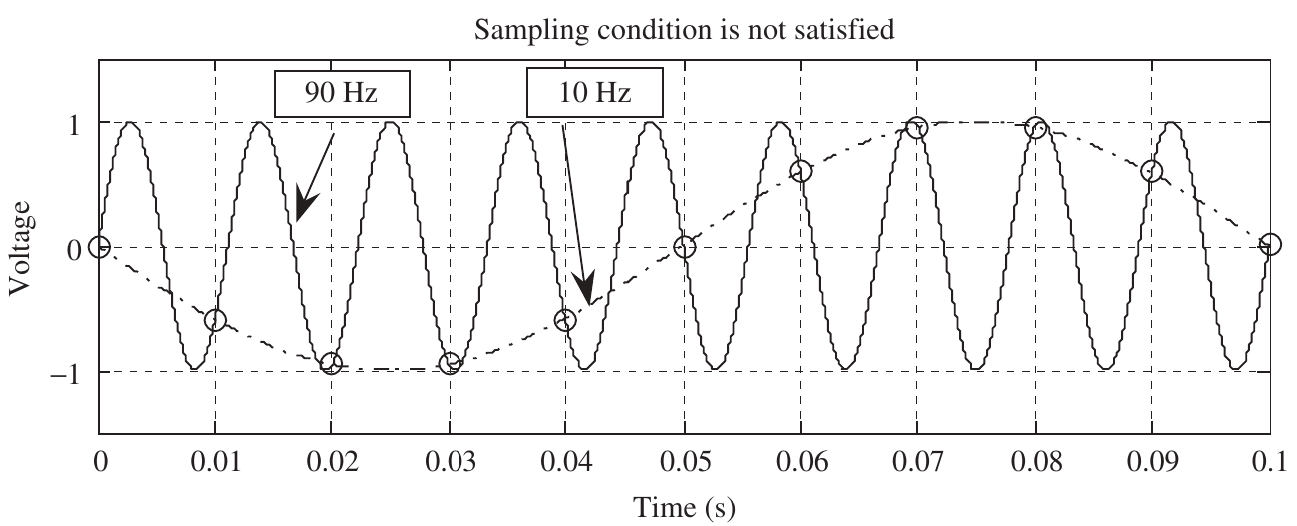
\includegraphics[width=0.9\linewidth]{./img/img05.png}
        \end{figure}
    \end{itemize}
\end{frame}

\begin{frame}{Sampling rate}
    \begin{itemize}
        \item What is minimum sampling rate?
        \begin{multicols}{2}
            \begin{enumerate}
                \item[a.] 500 Hz
                \item[b.] 1000 Hz
                \columnbreak
                \item[c.] 1500 Hz
                \item[d.] 2000 Hz
            \end{enumerate}
        \end{multicols}
        \begin{figure}
            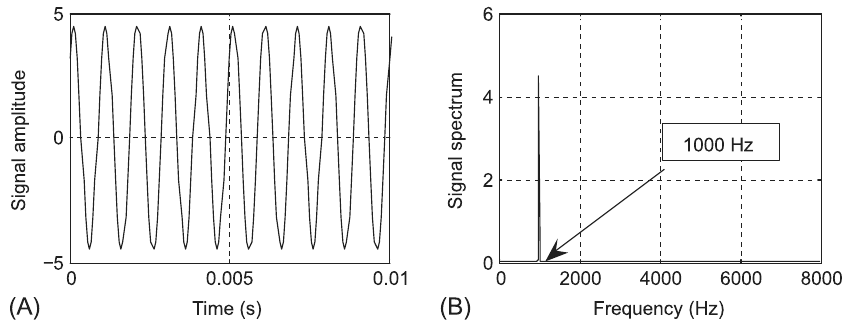
\includegraphics[width=\linewidth]{./img/img06}
        \end{figure}
    \end{itemize}
\end{frame}

\begin{frame}{Sampling rate}
    \begin{itemize}
        \item What is minimum sampling rate?
        \begin{multicols}{2}
            \begin{enumerate}
                \item[a.] 2000 Hz
                \item[b.] 4000 Hz
                \columnbreak
                \item[c.] 6000 Hz
                \item[d.] 8000 Hz
            \end{enumerate}
        \end{multicols}
        \begin{figure}
            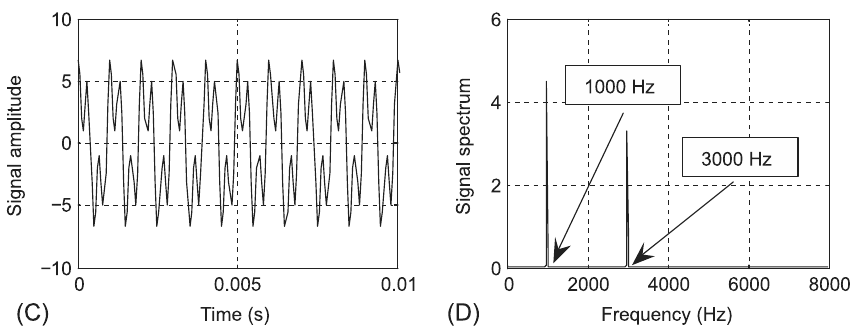
\includegraphics[width=\linewidth]{./img/img07}
        \end{figure}
    \end{itemize}
\end{frame}

\begin{frame}{The simplified sampling process}
    \begin{itemize}
        \item The sampled signal $x_s(t)$ obtained by sampling the continuous signal $x(t)$ at a sampling rate of $f_s$ samples per second
    \end{itemize}
    \begin{figure}
        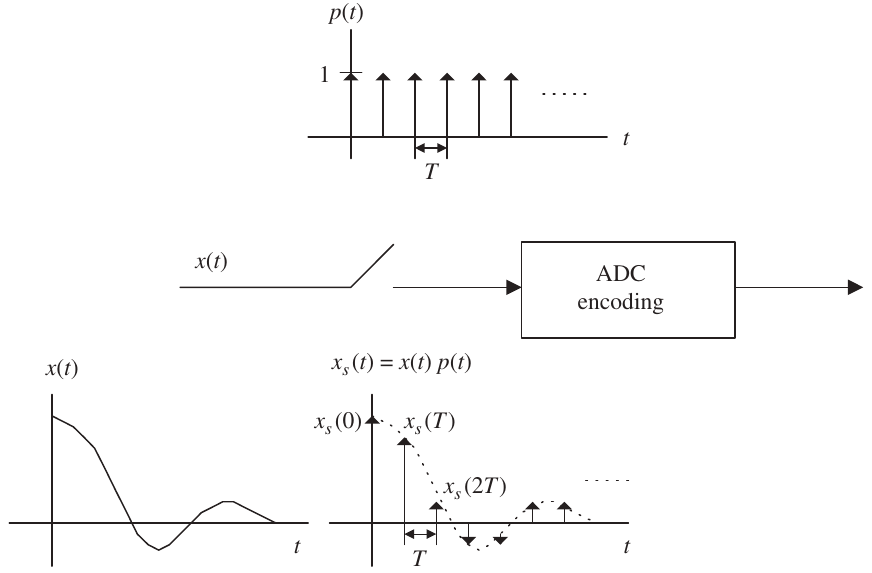
\includegraphics[width=0.8\linewidth]{./img/img08}
    \end{figure}
\end{frame}

\begin{frame}{Sampling process}
    \begin{itemize}
        \item Sampling process can be written as the product of the continuous signal and the sampling pulses (pulse train) with a period $T = 1/f_s$
        \begin{equation}
            x_s(t) = x(t) p(t)
            \label{eq:xs}
        \end{equation}
        \item The pulse train can be expressed as
        \begin{equation}
            p(t) = \sum_{n = - \infty}^\infty \delta(t - nT)
        \end{equation}
    \end{itemize}
\end{frame}

\begin{frame}{Sampling process}
    \begin{itemize}
        \item $p(t)$ with a fundamental frequency of $\omega_0 = 2\pi/T = 2\pi f_s$ rad/s. can be expanded by the Fourier series:
        \begin{equation}
            p(t) = \sum_{k = - \infty}^\infty a_k e^{jk\omega_0t}
            \label{eq:pt_deret}
        \end{equation}
        where $a_k$ are the Fourier coefficients which can be determined by
        \begin{equation}
            a_k = \frac{1}{T} \int_{-\infty}^{\infty} \delta(t)e^{-jk\omega_0t}dt = \frac{1}{T}
            \label{eq:keof.Fourier}
        \end{equation}
    \end{itemize}
\end{frame}

\begin{frame}{Sampling process}
    \begin{itemize}
        \item Substituting Eq. (\ref{eq:keof.Fourier}) into Eq. (\ref{eq:pt_deret}), the pulse train is given by
        \begin{equation}
            p(t) = \sum_{k = -\infty}^{\infty} \frac{1}{T} e^{jk\omega_0t}
            \label{eq:pt_new}
        \end{equation}
        \item Again, substituting Eq. (\ref{eq:pt_new}) into Eq. (\ref{eq:xs}),  leads to
        \begin{equation}
            x_s(t) = \sum_{k = -\infty}^{\infty} \frac{1}{T} x(t) e^{jk\omega_0t}
            \label{eq:xs_new}
        \end{equation}
    \end{itemize}
\end{frame}

\begin{frame}{Sampling process}
    \begin{itemize}
        \item Applying Fourier transform on Eq. (\ref{eq:xs_new}):
        \begin{equation}
            \begin{aligned}[b]
                X_s(f) &= \text{FT} \left\{ \sum_{k = -\infty}^{\infty} \frac{1}{T} x(t) e^{jk\omega_0t} \right\} \\
                &= \sum_{k = -\infty}^{\infty} \frac{1}{T} \text{ FT} \left\{ x(t) e^{jk\omega_0t} \right\} \\
                &= \sum_{k = -\infty}^{\infty} \frac{1}{T} \int_{-\infty}^{\infty} \left\{ x(t) e^{jk\omega_0t} \right\}e^{-j\omega t} dt
            \end{aligned}
        \end{equation}
    \end{itemize}
\end{frame}

\begin{frame}{Sampling process}
    \begin{itemize}
        \item that is,
        \begin{equation}
            \begin{aligned}[b]
                X_s(f) &= \sum_{k = -\infty}^{\infty} \frac{1}{T} \int_{-\infty}^{\infty} x(t) e^{-j(\omega-k\omega_0) t} dt \\
                 &= \sum_{k = -\infty}^{\infty} \frac{1}{T} \int_{-\infty}^{\infty} x(t) e^{-j2\pi(f-kf_s) t} dt
                \label{eq:Xsf}
            \end{aligned}
        \end{equation}
    \end{itemize}
\end{frame}

\begin{frame}{Sampling process}
    \begin{itemize}
        \item From the definition of Fourier transform, we note that
        \begin{equation}
            X(f) = \sum_{k = -\infty}^{\infty} \frac{1}{T} \int_{-\infty}^{\infty} x(t) e^{-j2\pi ft} dt
            \label{eq:Xf}
        \end{equation}
    \end{itemize}
\end{frame}

\begin{frame}{Sampling process}
    \begin{itemize}
        \item Using Eq. (\ref{eq:Xf}), the original spectrum (frequency components) $X(f)$ and the sampled signal spectrum $X_s(f)$ in terms of Hz are related as
        \begin{equation}
            X_s(f) = \frac{1}{T} \sum_{k = -\infty}^{\infty} X(f - kf_s)
            \label{eq:Xsf_and_Xf}
        \end{equation}
        where $X(f)$ is assumed to be the original baseband spectrum while $X_s(f)$ is its sampled signal spectrum, consisting of the original baseband spectrum $X(f)$ and its replicas $X(f\pm kf_s)$
    \end{itemize}
\end{frame}

\begin{frame}{Sampling process}
    \begin{itemize}
        \item Expanding Eq. (\ref{eq:Xsf_and_Xf}) leads to the sampled signal spectrum
        \begin{equation}
            X_s(f) = \cdots + \frac{1}{T}X(f+f_s) + \frac{1}{T}X(f) + \frac{1}{T}X(f-f_s) + \cdots
            \label{eq:deret_Xsf_and_Xf}
        \end{equation}
        \item Eq. (\ref{eq:deret_Xsf_and_Xf}) indicates that the sampled signal spectrum is the sum of the scaled original spectrum and
        copies of its shifted versions, called replicas.
        \item Eq. (\ref{eq:deret_Xsf_and_Xf}) have three possible sketches.
    \end{itemize}
\end{frame}

\begin{frame}{Sampling process}
    \begin{itemize}
        \item Condition 1: Sampled signal spectrum for $f_s > 2B$
        \begin{figure}
            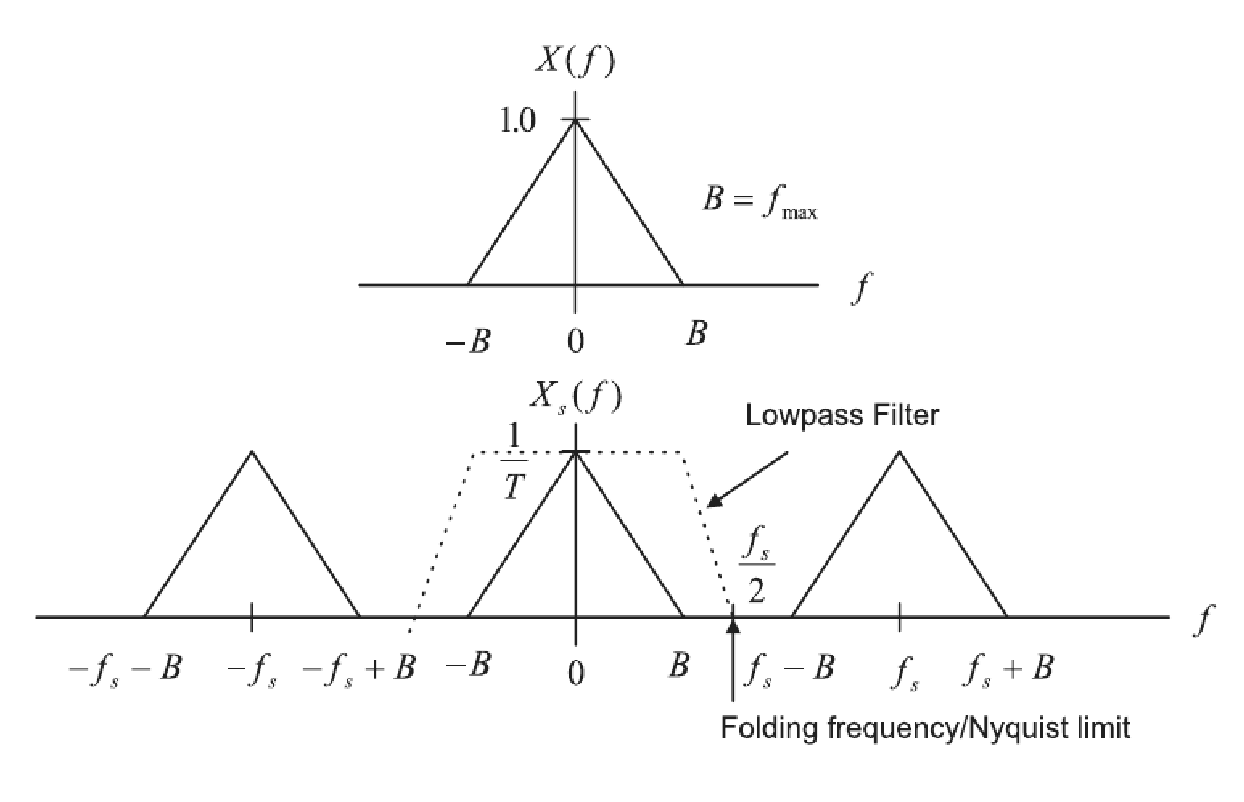
\includegraphics[width=0.9\linewidth]{./img/img09}
            \label{img:09}
        \end{figure}
    \end{itemize}
\end{frame}

\begin{frame}{Sampling process}
    \begin{itemize}
        \item Condition 2: Sampled signal spectrum for $f_s = 2B$
        \begin{figure}
            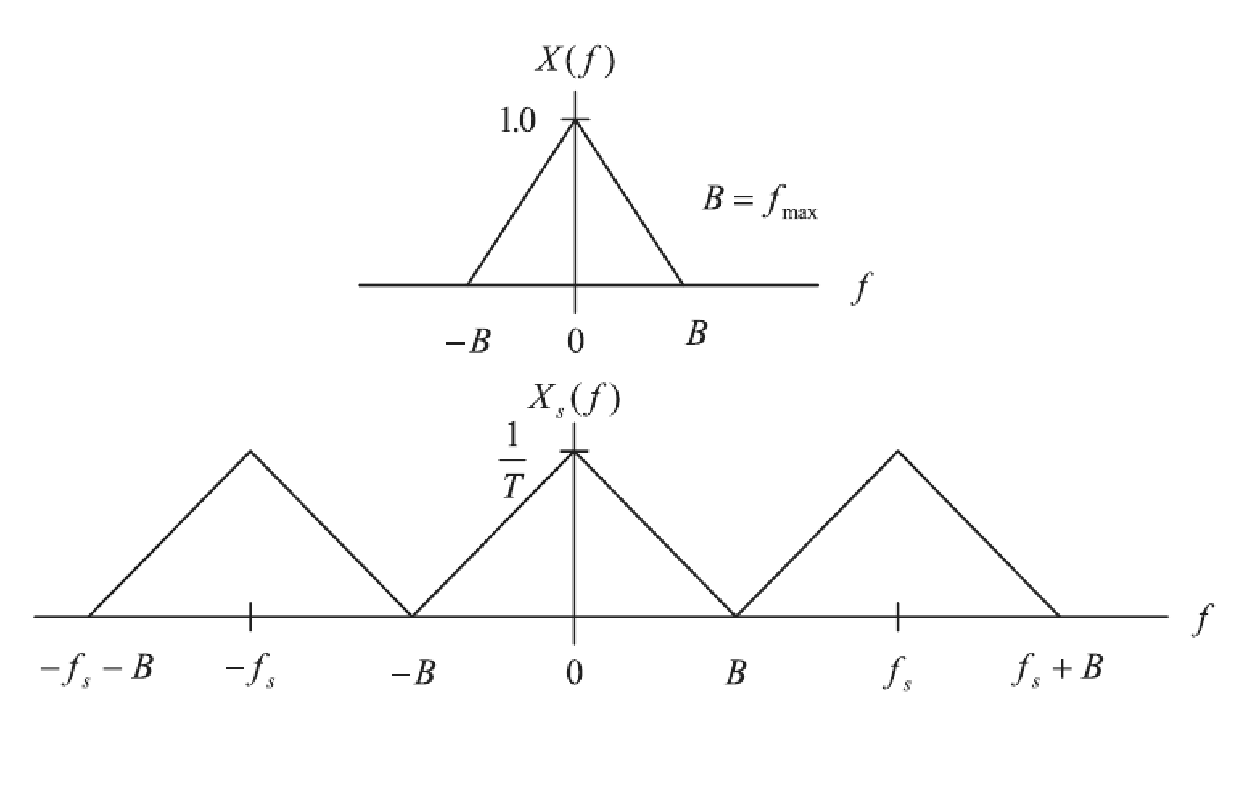
\includegraphics[width=0.9\linewidth]{./img/img10}
        \end{figure}
    \end{itemize}
\end{frame}

\begin{frame}{Sampling process}
    \begin{itemize}
        \item Condition 3: Sampled signal spectrum for $f_s < 2B$
        \begin{figure}
            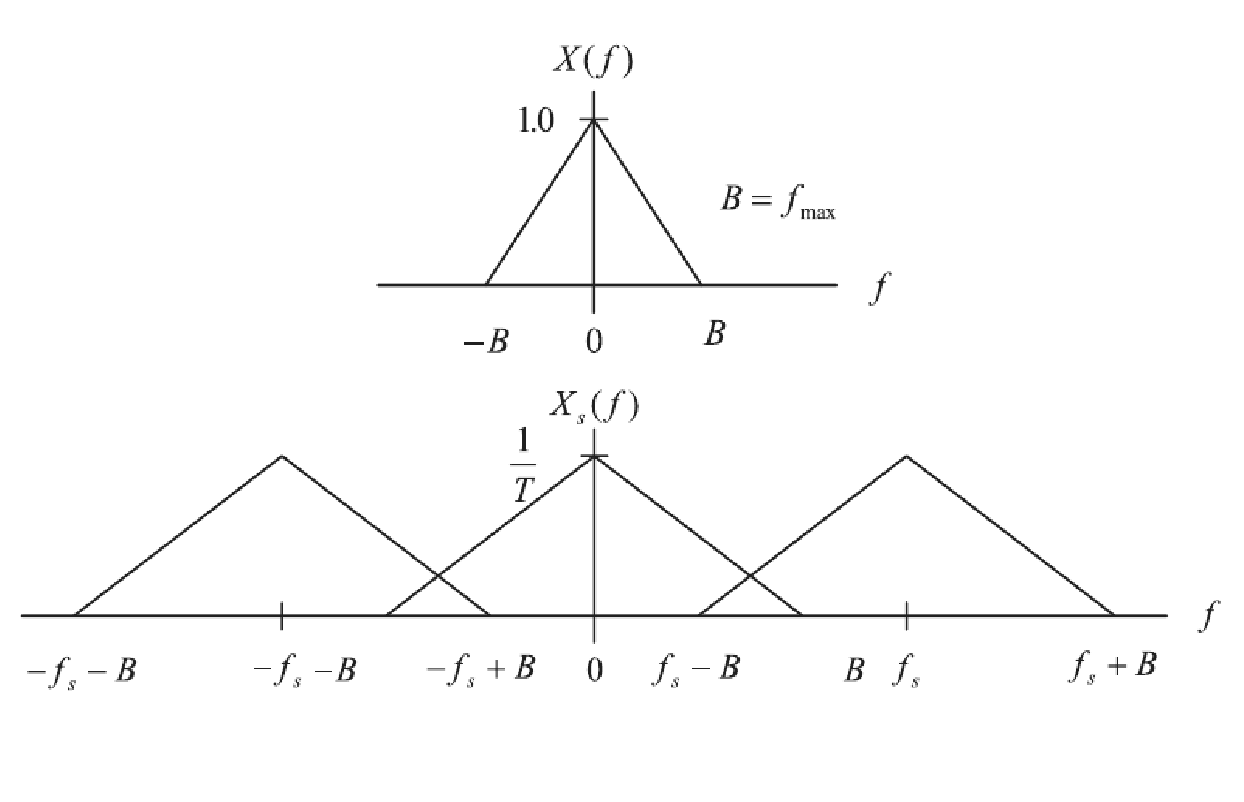
\includegraphics[width=0.9\linewidth]{./img/img11}
        \end{figure}
    \end{itemize}
\end{frame}

\begin{frame}{Sampling process}
    \begin{itemize}
        \item If applying a lowpass reconstruction filter to obtain exact reconstruction of the original signal spectrum, the following condition must be satisfied:
        \begin{equation}
            f_s - f_{\text{max}} \geq f_{\text{max}}
            \label{eq:2.12}
        \end{equation}
    \end{itemize} 
\end{frame}

\begin{frame}{Sampling process}
    \begin{itemize}
        \item Solving Eq. (\ref{eq:2.12}) gives
        \begin{equation}
            f_s \geq 2f_{\text{max}}
            \label{eq:freq_nyquist}
        \end{equation}
        \item In terms of frequency in radians per second, Eq. (\ref{eq:freq_nyquist}) is equivalent to
        \begin{equation}
            \omega_s \geq 2\omega_{\text{max}}
        \end{equation}
        \item This fundamental conclusion is well known as the \textbf{Shannon sampling theorem}
        \item Half of the sampling frequency $$ \frac{f_s}{2} \geq f_\text{max} $$ is usually called the \textbf{Nyquist frequency} (\textbf{Nyquist limit}) or \textbf{folding frequency}
    \end{itemize} 
\end{frame}

\begin{frame}{Shannon sampling theorem}
    \begin{theorem}
        For a uniformly sampled DSP system, an analog signal can be perfectly recovered as long as the sampling rate is at least twice as large as the highest-frequency component of the analog signal to be sampled.
    \end{theorem}
\end{frame}

\begin{frame}{Example 1}
    \begin{enumerate}
        \item Suppose that an analog signal is given as
        \begin{equation*}
            x(t) = 5 \cos (2 \pi 1000 t),~\text{ untuk } t \geq 0
        \end{equation*}
        and is sampled at the rate 8000 Hz
        \begin{enumerate}
            \item[a.] Sketch the spectrum for the original signal, $X(f)$
            \item[b.] Sketch the spectrum for the sampled signal from 0 to 20 kHz, $X_s(f)$
        \end{enumerate}
    \end{enumerate}
\end{frame}

\begin{frame}{Solution}
    \begin{itemize}
        \item Since the analog signal is sinusoid with a peak value of 5 and frequency of 1000 Hz, we can write the sine wave using Euler's identity:
    \end{itemize}
    \begin{framed}
    \textbf{Euler's identity}
        \begin{align}
            \sin(x) = \frac{(e^{jx} - e^{-jx})}{2j} \\
            \cos(x) = \frac{(e^{jx} + e^{-jx})}{2}
        \end{align}
    \end{framed}
\end{frame}

\begin{frame}{Solution}
    \begin{itemize}
        \item therefore
        \begin{align*}
            x(t) &= 5 \cos (2 \pi 1000 t) = 5 \left( \frac{(e^{j2\pi 1000t} + e^{-j2\pi 1000t})}{2} \right) \\
            &= 2.5 e^{j2 \pi 1000t} + 2.5 e^{-j2 \pi 1000t}
            \label{eq:lat.soal.1}
        \end{align*}
        is a Fourier series expansion for a continuous periodic signal in terms of the exponential form
    \end{itemize}
    \begin{framed}
        \textbf{Fourier series expansion in terms of the exponential form:}
        \begin{equation*}
            x(t) = \sum_{k=-\infty}^{-\infty} c_k e^{jk\omega_0 t} = \sum_{k=-\infty}^{-\infty} c_k e^{jk 2\pi f_0 t}
        \end{equation*}
    \end{framed}
\end{frame}

\begin{frame}{Solution}
    \begin{itemize}
        \item We can identify the Fourier series coefficients as
        \begin{align*}
            c_1 &= 2.5 \\
            &\text{ and }\\
            c_{-1} &= 2.5
        \end{align*}
        \item Using the magnitudes of the coefficients, we then plot the two-side spectrum
    \end{itemize}
\end{frame}

\begin{frame}{Solution}
    \begin{itemize}
        \item Spectrum of the analog signal $X(f)$
        \begin{figure}
            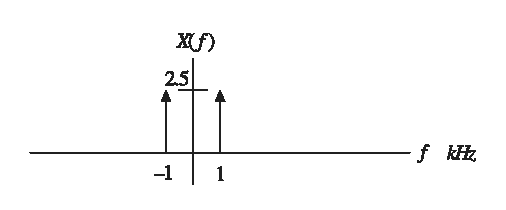
\includegraphics[width=\linewidth]{./img/img12}
        \end{figure}
    \end{itemize}
\end{frame}

\begin{frame}{Solution}
    \begin{itemize}
        \item After the analog signal is sampled at the rate of 8000 Hz, the sampled signal spectrum and its replicas centered at the frequencies $\pm kf_s$, each with the scaled amplitude being $2.5/T$
        \begin{figure}
            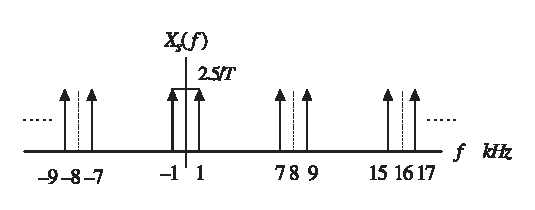
\includegraphics[width=\linewidth]{./img/img13}
        \end{figure}
    \end{itemize}
\end{frame}

\begin{frame}{Example 2}
    \begin{enumerate}
        \setcounter{enumi}{1}
        \item Suppose that an analog signal is given as
        \begin{equation*}
            x(t) = 5 \cos (2 \pi 1500 t),~\text{ untuk } t \geq 0
        \end{equation*}
        and is sampled at the rate 8000 Hz
        \begin{enumerate}
            \item[a.] Sketch the spectrum for the original signal, $X(f)$
            \item[b.] Sketch the spectrum for the sampled signal from 0 to 20 kHz, $X_s(f)$
        \end{enumerate}
    \end{enumerate}
\end{frame}

\begin{frame}{Example 3}
    \begin{enumerate}
        \setcounter{enumi}{2}
        \item Suppose that an analog signal is given as
        \begin{equation*}
            x(t) = 5 \cos (2 \pi 1500 t) + 2 \cos (2 \pi 2200 t),~\text{ untuk } t \geq 0
        \end{equation*}
        and is sampled at the rate 8000 Hz
        \begin{enumerate}
            \item[a.] Sketch the spectrum for the original signal, $X(f)$
            \item[b.] Sketch the spectrum for the sampled signal from 0 to 20 kHz, $X_s(f)$
        \end{enumerate}
    \end{enumerate}
\end{frame}

\begin{frame}{Example 4}
    \begin{enumerate}
        \setcounter{enumi}{3}
        \item Suppose that an analog signal is given as
        \begin{equation*}
            x(t) = 3 \cos (2 \pi 2500 t) + 2 \cos (2 \pi 4200 t),~\text{ untuk } t \geq 0
        \end{equation*}
        and is sampled at the rate 8000 Hz
        \begin{enumerate}
            \item[a.] Sketch the spectrum for the original signal, $X(f)$
            \item[b.] Sketch the spectrum for the sampled signal from 0 to 20 kHz, $X_s(f)$
        \end{enumerate}
    \end{enumerate}
\end{frame}

\end{document}